%%% In this section, you will describe all of the various artifacts that you will generate and maintain during the project life cycle. Describe the purpose of each item below, how the content will be generated, where it will be stored, how often it will be updated, etc. Replace the default text for each section with your own description. Reword this paragraph as appropriate.

\subsection{Major Documentation Deliverables}

\subsubsection{Project Charter}
The initial version of the Project Charter will be delivered on 10/8/2021, with a final draft of the initial document completed on 10/10/2021. After that, Lydia Sarver will be responsible for updating the document as needed for items changing. Some items that may change include:
\begin{itemize}
  \item Current and pending support
  \item Milestone date changes
\end{itemize}
\\
The absolute final version of this document will be completed on or before the Final Project Demonstration Day, which is to be held in May 2022.

\subsubsection{System Requirements Specification}
The initial version of the System Requirements Specification document will be completed on 10/22/2021, with a final draft of the initial document completed on 10/24/2021. The team will be responsible for updating this document if the requirement they are working on at the time has to be changed for any reason. The absolute final version of this document will be completed on or before the Final Project Demonstration Day, which is to be held in May 2022.

\subsubsection{Architectural Design Specification}
The initial version of the Architectural Design Specification document will be completed on 11/12/2021, with a final draft of the initial document completed on 11/14/2021. The team will be responsible for updating this document if the design specification they are working on at the time has to be changed for any reason.  The absolute final version of this document will be completed on or before the Final Project Demonstration Day, which is to be held in May 2022.

\subsubsection{Detailed Design Specification}
The initial version of the Detailed Design Specification document will be completed on (Friday before due date), with a final draft of the initial document completed on (Sunday before due date). The team will be responsible for updating this document if the design specification they are working on at the time has to be changed for any reason and as the design becomes more detailed. The absolute final version of this document will be completed on or before the Final Project Demonstration Day, which is to be held in May 2022.

\subsection{Recurring Sprint Items}

\subsubsection{Product Backlog}
After we decide the items for the System Requirements Specification document, they will be added to our Jira project (the software we are using to monitor our sprints and sprint items). The items will be prioritized by people's availability and group vote as to what is the next most important items. If multiple people have a large availability during a given sprint, multiple items can be worked on during said sprint.

\subsubsection{Sprint Planning}
Each sprint will be planned the week between sprints during our weekly group meetings. We will look through our backlog, consider what the best next steps are and what assignment is due next, and decide accordingly. We will have 9 sprints during our project.

\subsubsection{Sprint Goal}
We will decide the sprint goal based off of the next best step for our project as well as the assignment due dates for our Senior Design Class. This goal will be decided on as a group. We do not have a customer to involve in this process.

\subsubsection{Sprint Backlog}
The sprint backlog will be decided by the sprint goal and what tasks are both applicable to achieving the goal and feasible for the two week time frame. We are using Jira to maintain our sprint backlog as well as our Scrum board.

\subsubsection{Task Breakdown}
Individual tasks from the sprint backlog will be on a volunteer basis originally, but the Scrum Master may ask or delegate tasks as needed. The time we spend on tasks will be documented in Story Points because of the limitations of Jira. However, each story point will represent 30 minute intervals.

\subsubsection{Sprint Burn Down Charts}
Burn down charts will be produced by the Scrum Master at the end of each Sprint. Each group member will be responsible for estimating and tracking the time spent for each of their Sprint Issues. The burn down chart will be provided in the format Jira provides. The burn down chart for Sprint 2 will be added to this document as an example after it is created.

%%%%%%%%%%%%%%%%%%%%%%%%%%%%%%%%%%%%%%%%%%%%%%%%%%%%%%%%%%
%  BE SURE TO UPDATE THE IMAGE CAPTION
%\begin{figure}[h!]
%    \centering
%    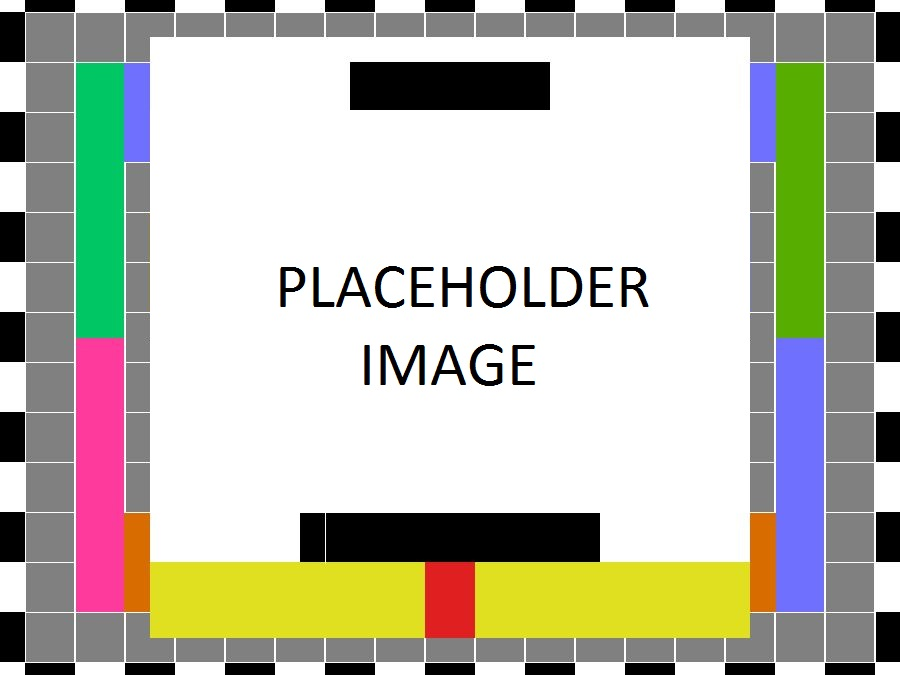
\includegraphics[width=0.5\textwidth]{images/test_image} % Image
%    \caption{Example sprint burn down chart} % Caption
%\end{figure}

\subsubsection{Sprint Retrospective}
Our sprint retrospective will be held as an agenda point during our weekly meeting we will hold in between sprints. We will discuss what we finished, what was left, what we did well as a group and as individuals, as well as what we did not do well as a group and as individuals. We will document these in the notes we take for all of our meetings. Before this meeting, each member will be encouraged to consider these topics and bring them with them to that meeting. 
\subsubsection{Individual Status Reports}
Individual status reports will be produced at the end of each Sprint. Key items reported in this are:
\begin{itemize}
  \item Previous Sprint's Goal
  \item Previous Sprint's Backlog
  \item Individual Time Expenditures
  \item Team Burn Down Chart [Not relevant for Sprint 1]
  \item Individual Retrospective
  \item Peer Review
\end{itemize}

\subsubsection{Engineering Notebooks}
Our engineering notebooks will be updated everyday we do anything with the project. This should take place at least once a week, but will all most certainly happen more often. We will not keep a page number requirement for each person. They should track what is important to our project and the amount of pages required is expected to be different for each person. The engineering notebooks will be due in class periodically throughout the two semesters. We will sign off on each other's notebook pages as witnesses, but each person will be responsible for keeping up with their own notebook.

\subsection{Closeout Materials}

\subsubsection{System Prototype}
Our final system prototype will be an autonomous longboard as well as a web app remote. This final prototype will be demonstrated prior to the Senior Design Final Presentation day and videotaped to be shown to the reviewers due to safety concerns. There will not be any Prototype Acceptance Tests or Field Acceptance Tests.

\subsubsection{Project Poster}
Our poster will be a tri-fold board will be 48" x 36". It will be delivered on the CoE Innovation Day poster presentation as well as the Final Senior Design Presentation Day. It will have our board design schematic, a few specific parts of the board's schematics, and some problems we faced when building it. In front of our poster, we will have a laptop paying a soundless video of our longboard in use.


\subsubsection{Web Page}
Our web page will hold our web app when viewed on a mobile device. However, when viewed on a desktop pages about our board design, team, and more things to be decided at a later date will be found. Our final web page will be published in May of 2022. We will update the drafted version as we continue to develop our project, however the final web page will not be complete until May 2022. Sahaj Amatya will be in charge of updating our web page.

\subsubsection{Demo Video}
Our demo video will show our longboard in action with someone riding it, the board following someone, and it navigating to someone. We plan to include B-roll footage for future video cuts for the CSE department. The videos will be less than a minute in length and cover topics including autonomy, path finding, and turning mechanisms.

\subsubsection{Source Code}
Our source code is being maintained on GitHub. We will use their version control system. Our source code will not be open source.

\subsubsection{Source Code Documentation}
Our final documentation will be available in PDF format. We are following good code practices to ensure clean and understandable comments for our code.

\subsubsection{Hardware Schematics}
We will be wiring our components together. As we get our schematics for these wiring diagrams, they will be listed here.

\subsubsection{CAD files}
Our project will require mechanical design. We are using SolidWorks and TinkerCAD.
Our closeout materials will be provided in OBJ, STL, and MTL files.

\subsubsection{Installation Scripts}
Our project will not require installation scripts. The board will already have the program to run it installed and the app is a web app and therefore updated on the server side of the app.

\subsubsection{User Manual}
We will provide a digital user manual for board and app use. It will walk the user through general setup of the board and how to use the web app.
